\documentclass[a4paper,12pt,twoside]{memoir}

% Castellano
\usepackage[spanish,es-tabla]{babel}
\selectlanguage{spanish}
\usepackage[utf8]{inputenc}
\usepackage[T1]{fontenc}
\usepackage{lmodern} % Scalable font
\usepackage{microtype}
\usepackage{placeins}

\RequirePackage{booktabs}
\RequirePackage[table]{xcolor}
\RequirePackage{xtab}
\RequirePackage{multirow}

% Links
\PassOptionsToPackage{hyphens}{url}\usepackage[colorlinks]{hyperref}
\hypersetup{
	allcolors = {red}
}

% Ecuaciones
\usepackage{amsmath}

% Rutas de fichero / paquete
\newcommand{\ruta}[1]{{\sffamily #1}}

% Párrafos
\nonzeroparskip

% Huérfanas y viudas
\widowpenalty100000
\clubpenalty100000

\let\tmp\oddsidemargin
\let\oddsidemargin\evensidemargin
\let\evensidemargin\tmp
\reversemarginpar

% Imágenes

% Comando para insertar una imagen en un lugar concreto.
% Los parámetros son:
% 1 --> Ruta absoluta/relativa de la figura
% 2 --> Texto a pie de figura
% 3 --> Tamaño en tanto por uno relativo al ancho de página
\usepackage{graphicx}

\newcommand{\imagen}[3]{
	\begin{figure}[!h]
		\centering
		\includegraphics[width=#3\textwidth]{#1}
		\caption{#2}\label{fig:#1}
	\end{figure}
	\FloatBarrier
}







\graphicspath{ {./img/} }

% Capítulos
\chapterstyle{bianchi}
\newcommand{\capitulo}[2]{
	\setcounter{chapter}{#1}
	\setcounter{section}{0}
	\setcounter{figure}{0}
	\setcounter{table}{0}
	\chapter*{#2}
	\addcontentsline{toc}{chapter}{#2}
	\markboth{#2}{#2}
}

% Apéndices
\renewcommand{\appendixname}{Apéndice}
\renewcommand*\cftappendixname{\appendixname}

\newcommand{\apendice}[1]{
	%\renewcommand{\thechapter}{A}
	\chapter{#1}
}

\renewcommand*\cftappendixname{\appendixname\ }

% Formato de portada

\makeatletter
\usepackage{xcolor}
\newcommand{\tutor}[1]{\def\@tutor{#1}}
\newcommand{\tutorb}[1]{\def\@tutorb{#1}}

\newcommand{\course}[1]{\def\@course{#1}}
\definecolor{cpardoBox}{HTML}{E6E6FF}
\def\maketitle{
  \null
  \thispagestyle{empty}
  % Cabecera ----------------
\begin{center}
  \noindent\includegraphics[width=\textwidth]{cabeceraSalud}\vspace{1.5cm}%
\end{center}
  
  % Título proyecto y escudo salud ----------------
  \begin{center}
    \begin{minipage}[c][1.5cm][c]{.20\textwidth}
        \includegraphics[width=\textwidth]{escudoSalud.pdf}
    \end{minipage}
  \end{center}
  
  \begin{center}
    \colorbox{cpardoBox}{%
        \begin{minipage}{.8\textwidth}
          \vspace{.5cm}\Large
          \begin{center}
          \textbf{TFG del Grado en Ingeniería de la Salud}\vspace{.6cm}\\
          \textbf{\LARGE\@title{}}
          \end{center}
          \vspace{.2cm}
        \end{minipage}
    }%
  \end{center}
  
    % Datos de alumno, curso y tutores ------------------
  \begin{center}%
  {%
    \noindent\LARGE
    Presentado por \@author{}\\ 
    en Universidad de Burgos\\
    \vspace{0.5cm}
    \noindent\Large
    \@date{}\\
    \vspace{0.5cm}
    %Tutor: \@tutor{}\\ % comenta el que no corresponda
    Tutores: \@tutor{} -- \@tutorb{}\\
  }%
  \end{center}%
  \null
  \cleardoublepage
  }
\makeatother

\newcommand{\nombre}{Pepe Pérez}
\newcommand{\nombreTutor}{Tutor 1} 
\newcommand{\nombreTutorb}{Tutor 2} 
\newcommand{\dni}{123456A} 

% Datos de portada
\title{Título del trabajo}
\author{\nombre}
\tutor{\nombreTutor}
\tutorb{\nombreTutorb}
\date{\today}


\begin{document}

\maketitle


\newpage\null\thispagestyle{empty}\newpage

%%%%%%%%%%%%%%%%%%%%%%%%%%%%%%%%%%%%%%%%%%%%%%%%%%%%%%%%%%%%%%%%%%%%%%%%%%%%%%%%%%%%%%%%
\thispagestyle{empty}


\noindent\includegraphics[width=\textwidth]{cabeceraSalud}\vspace{1cm}

\noindent D. \nombreTutor, profesor del departamento de departamento, área de área.

\noindent Expone:

\noindent Que el alumno D. \nombre, con DNI \dni, ha realizado el Trabajo final de Grado en Ingeniería de la Salud titulado título del trabajo. 

\noindent Y que dicho trabajo ha sido realizado por el alumno bajo la dirección del que suscribe, en virtud de lo cual se autoriza su presentación y defensa.

\begin{center} %\large
En Burgos, {\large \today}
\end{center}

\vfill\vfill\vfill

% Author and supervisor
\begin{minipage}{0.45\textwidth}
\begin{flushleft} %\large
Vº. Bº. del Tutor:\\[2cm]
D. \nombreTutor
\end{flushleft}
\end{minipage}
\hfill
\begin{minipage}{0.45\textwidth}
\begin{flushleft} %\large
Vº. Bº. del Tutor:\\[2cm]
D. \nombreTutorb
\end{flushleft}
\end{minipage}
\hfill

\vfill

% para casos con solo un tutor comentar lo anterior
% y descomentar lo siguiente
%Vº. Bº. del Tutor:\\[2cm]
%D. nombre tutor


\newpage\null\thispagestyle{empty}\newpage




\frontmatter

% Abstract en castellano
\renewcommand*\abstractname{Resumen}
\begin{abstract}
En este primer apartado se hace una \textbf{breve} presentación del tema que se aborda en el proyecto.
\end{abstract}

\renewcommand*\abstractname{Descriptores}
\begin{abstract}
Palabras separadas por comas que identifiquen el contenido del proyecto Ej: servidor web, buscador de vuelos, android \ldots
\end{abstract}

\clearpage

% Abstract en inglés
\renewcommand*\abstractname{Abstract}
\begin{abstract}
A \textbf{brief} presentation of the topic addressed in the project.
\end{abstract}

\renewcommand*\abstractname{Keywords}
\begin{abstract}
keywords separated by commas.
\end{abstract}

\clearpage

% Indices
\tableofcontents

\clearpage

\listoffigures

\clearpage

\listoftables
\clearpage


\mainmatter
\capitulo{1}{Objetivos}

Objetivos principales del trabajo realizado.

Este apartado explica de forma precisa y concisa cuales son los objetivos que se persiguen con la realización del proyecto. Se puede distinguir entre:
\begin{enumerate}
    \item Los objetivos marcados por los requisitos del software/hardware/análisis a desarrollar.
    \item Los objetivos de carácter técnico, relativos a la calidad de los resultados, velocidad de ejecución, fiabilidad o similares.
    \item Los objetivos de aprendizaje, relativos a aprender técnicas o herramientas de interés. 
\end{enumerate}









\capitulo{2}{Introducción} \label{Intro}

\setlength{\parskip}{10pt}

Una de las ventajas que presentan titulaciones como Ingeniería de la Salud es la capacidad para desarrollar proyectos interdisciplinares, es decir, que aúnen técnicas y conocimientos de diversos campos. Ejemplo de ello es el trabajo recogido en esta memoria, ya que en él convergen ideas pertenecientes al ámbito sanitario, biológico y computacional.

Este tipo de iniciativas son capaces de abrir nuevos campos de investigación, ampliar las perspectivas y mejorar la eficiencia en la resolución de problemas. Sin embargo, estas propuestas generalmente son complicadas de entender en su totalidad, debido a la heterogeneidad de conceptos abarcados.

Es por ello que en las siguientes secciones y subsecciones se van a explicar los fundamentos informáticos y fisiológicos esenciales para poder entender el proyecto, independientemente del ámbito al que pertenezca el lector, así como la estructura de la memoria y del resto de materiales entregados.

\titlespacing{\section}{0pt}{0.25cm}{0.15cm}
\section{Estructura de la memoria}

En este documento y sus correspondientes anexos se recoge toda la información del proyecto \textit{Detección del grado de retinopatía diabética mediante redes convolucionales}.

En la memoria principal se incluyen los capítulos detallados en el \hyperref[toc]{Índice}: \hyperref[Obj]{Objetivos}, \hyperref[Intro]{Introducción}, \hyperref[Met]{Metodología}, \hyperref[Conc]{Conclusiones}, \hyperref[Aspe]{Aspectos relevantes del desarrollo del proyecto} y \hyperref[Fut]{Líneas futuras}. Además se incluye la correspondiente bibliografía en la que se citan todas las fuentes empleadas en el proyecto.

Asimismo se entrega una memoria de anexos, que contiene materiales adicionales y ampliaciones de los contenidos de la memoria principal.

Todos los materiales empleados en el proyecto, incluyendo el código \LaTeX de las memorias, los scripts de Python para la creación y entrenamiento de modelos, y las imágenes empleadas en el entrenamiento, pueden encontrarse en el siguiente repositorio de GitHub: \href{https://github.com/SamuelLozanoJuarez/CNN_and_Diabetic_Retinopathy}{CNN and Diabetic Retinopathy}.

\titlespacing{\section}{0pt}{0.25cm}{0.15cm}
\section{Conceptos teóricos básicos}

A continuación se van a explicar los conceptos teóricos fundamentales sobre la retinopatía diabética y las redes neuronales convolucionales, necesarios para entender el contexto en que se desarrolla este proyecto.

\titlespacing{\subsection}{0pt}{0.25cm}{0.15cm}
\subsection{Retinopatía diabética}

La retinopatía diabética (RD) es la complicación más común de la diabetes mellitus (DM), y constituye una de las principales causas de ceguera en edad avanzada \cite{diabetes:JDI, retinopatia:Retinal_and_eye}. Se trata de una microangiopatía diabética, una patología que afecta a los capilares que irrigan la retina, como consecuencia de los altos niveles de glucosa en sangre \cite{retinopatia:chile}.

Esta enfermedad se desarrolla en más de una quinta parte de los individuos diagnosticados con DM a nivel global, siendo esta proporción mayor en la región de América del Norte. En números brutos estamos hablando de más de 100 millones de personas que padecen esta afección en todo el mundo \footnote{Los datos se corresponden con un estudio realizado en el año 2021.} \cite{retinopatia:ophtalmology}.

A pesar de que existen tratamientos que permiten ralentizar, e incluso revertir, la evolución de la enfermedad, estos presentan una mayor eficacia en las primeras etapas de desarrollo de la RD, por lo que un diagnóstico temprano es fundamental a la hora de preservar la visión del paciente \cite{diabetes:JDI}.

\subsubsection{Sub Subsección}

\subsection{Redes Neuronales Convolucionales}

En esta sección y el resto de secciones de la memoria puede ser necesario incluir listas de items.

\begin{itemize}
    \item item1
    \item item2
    \item item3
\end{itemize}

Listas enumeradas.

\begin{enumerate}
    \item item1
    \item item2
    \item item3
\end{enumerate}

Figuras, como la figura \ref{fig:escudo} que aparece en la página \pageref{fig:escudo}. 

Puedes aprender más de las figuras en la dirección \url{https://es.overleaf.com/learn/latex/Inserting_Images}

\begin{figure}[h]
    \centering
    \includegraphics[width=0.25\textwidth]{img/escudoSalud.pdf}
    \caption{Pie de la figura}
    \label{fig:escudo}
\end{figure}


También se pueden insertar tablas como \ref{tab:my-table}, que ha sido generada con \url{https://www.tablesgenerator.com/}.

\begin{table}[]
\begin{tabular}{lll}
a & b & c \\
1 & 2 & 3 \\
4 & 5 & 6
\end{tabular}
\caption{}
\label{tab:my-table}
\end{table}

Es necesario que todas las figuras y tablas aparezca referenciadas en el texto, como estos ejemplos.

Todos los conceptos teóricos deben de estar correctamente referenciados en la bibliografía. Por ejemplo, aquí estoy citando la página de \LaTeX{} de Wikipedia \cite{wiki:latex}.

También puede ser necesario utilizar notas al pie \footnote{como por ejemplo esta}, para aclarar algunos conceptos.

\section{Marco de trabajo}

\section{Estado del arte y trabajos relacionados}

En este apartado sería interesante también incluir la justificación del proyecto, qué se pretende hacer en este proyecto que no se haya hecho en otros, qué es lo novedoso que se va a introducir (en este caso adecuar la red para que trabaje sobre imágenes de dispositivos móviles en vez de imágenes de OCT).

Revisión bibliográfica de que se está haciendo en la industria o la academia relativo al problema que se está tratando.

Enumeración y resumen de todos los trabajos relacionados de interés.


\capitulo{3}{Metodología} \label{Met}

\titlespacing{\section}{0pt}{0.25cm}{0.15cm}
\section{Descripción de los datos.}

Para el entrenamiento de los distintos modelos planteados se han usado dos conjuntos de datos. El primero de ellos, proporcionado por el Departamento de Ciencias de la Salud de la Universidad de Burgos, corresponde a una cohorte local de Burgos. El segundo está formado por imágenes obtenidas de distintos repositorios públicos a nivel global.

\subsection{Cohorte local}

El primer conjunto de datos del que se dispuso para la realización del proyecto fue proporcionado por el Departamento de Ciencias de la Salud de la Universidad de Burgos. Este conjunto está compuesto por un total de 510 imágenes y un archivo Excel: \textit{Calidad\_Diagnóstico\_Fotos.xlsx}. Cada una de las imágenes fue evaluada por dos oftalmólogos distintos para determinar el grado de RD correspondiente.

Los pacientes a los que corresponde la información fueron obtenidos de las consultas de oftalmología de la sección de diabetes del Servicio de Oftalmología del Hospital Universitario de Burgos (HUBU). Como criterios de inclusión se tuvo en cuenta que los pacientes fueran mayores de 18 años, sin contraindicaciones para la midriasis farmacológica con tropicamida o fenilefrina.

En el archivo Excel cada uno de los registros representa una imagen de las 510 entregadas. Los atributos del archivo almacenan información sobre distintas características de cada imagen. Los campos más relevantes, y que van a ser empleados a lo largo del proyecto, son:

\begin{enumerate}[itemsep=0.25em]
    \item \textit{NHC}: número entero que se corresponde con el número de historia clínica en el HUBU del paciente del que se obtuvo la imagen.
    \item \textit{1 OCT 2 IPHONE 3 SAMSUNG}: etiqueta que representa el dispositivo con el que se obtuvo la imagen. Puede tomar tres posibles valores: 1 si la imagen fue obtenida utilizando un tomógrafo de coherencia óptica (OCT por sus siglas en inglés), 2 si la imagen fue obtenida utilizando el dispositivo Ret-iN CaM acoplado a un teléfono iPhone y 3 si la imagen fue obtenida utilizando el mismo dispositivo acoplado a un teléfono Samsung.
    \item \textit{lateralidad 1 Dch 2 izq}: etiqueta que representa la lateralidad del ojo. Puede tomar dos posibles valores: 1 si la imagen se corresponde con el ojo derecho del paciente y 2 si la imagen se corresponde con el ojo izquierdo. 
    \item \textit{Retinologo 1 y 2}: etiqueta acerca el oftalmólogo que ha proporcionado el diagnóstico sobre esa imagen. Si toma valor 1 el diagnóstico que aparece en ese registro fue emitido por el primer oftalmólogo, si toma valor 2 fue emitido por el segundo oftalmólogo.
    \item \textit{CALIDAD GRAL IMAGEN}: evaluación de la calidad de la imagen. Puede tomar cinco valores: 1 si la calidad es no valorable, 2 si es deficiente, 3 si es media, 4 buena y 5 excelente.
    \item \textit{GRADO RETINOPATÍA DIABÉTICA}: diagnóstico proporcionado por el oftalmólogo. Si toma valor 1 la imagen es etiquetada como sana, 2 se corresponde con NPDR leve, 3 con NPDR moderada, 4 con NPDR severa y 5 se corresponde con PDR.
\end{enumerate}

Las 510 imágenes proporcionadas se distribuyeron entre los tres dispositivos de adquisición de la siguiente manera: 176 imágenes obtenidas con OCT, 171 con iPhone y 163 con Samsung. Las fotografías fueron realizadas bajo midriasis farmacológica usando el DRI OCT Triton, un Samsung Galaxy S7 y un iPhone 11 Pro \footnote{Si se desea más información acerca de los datos puede consultarse el anexo \textit{Descripción de adquisición y tratamiento de datos}}.

De todas las imágenes disponibles se eliminaron 205 por no estar etiquetadas o porque su calidad era inferior a 4, como se explicará en el siguiente apartado. La distribución entre dispositivos de adquisición y grados de RD, de las 305 imágenes restantes empleadas en el entrenamiento de los modelos, puede observarse en la tabla \ref{tab:cohorte}. En la figura \ref{fig:comp_dispositivos} pueden observarse las imágenes de retina de un mismo ojo sano (Grado 1) obtenidas con los distintos dispositivos. 

\begin{table}[h]
\centering
\begin{tabular}{@{}llllll|l@{}}
\toprule
\rowcolor[HTML]{C0C0C0}
        & G1 & G2 & G3  & G4 & G5 & Total \\ \midrule
OCT     & 25 & 20 & 58  & 4  & 6  & 113   \\
iPhone  & 22 & 13 & 48  & 8  & 8  & 99    \\
Samsung & 25 & 4  & 47  & 7  & 10 & 93    \\ \midrule
Total   & 72 & 37 & 153 & 19 & 24 & 305   \\ \bottomrule
\end{tabular}
\caption{Distribución de las imágenes de la cohorte local entre los distintos dispositivos (filas) y grados (columnas).}
\label{tab:cohorte}
\end{table}

\begin{figure}[h]
    \centering
    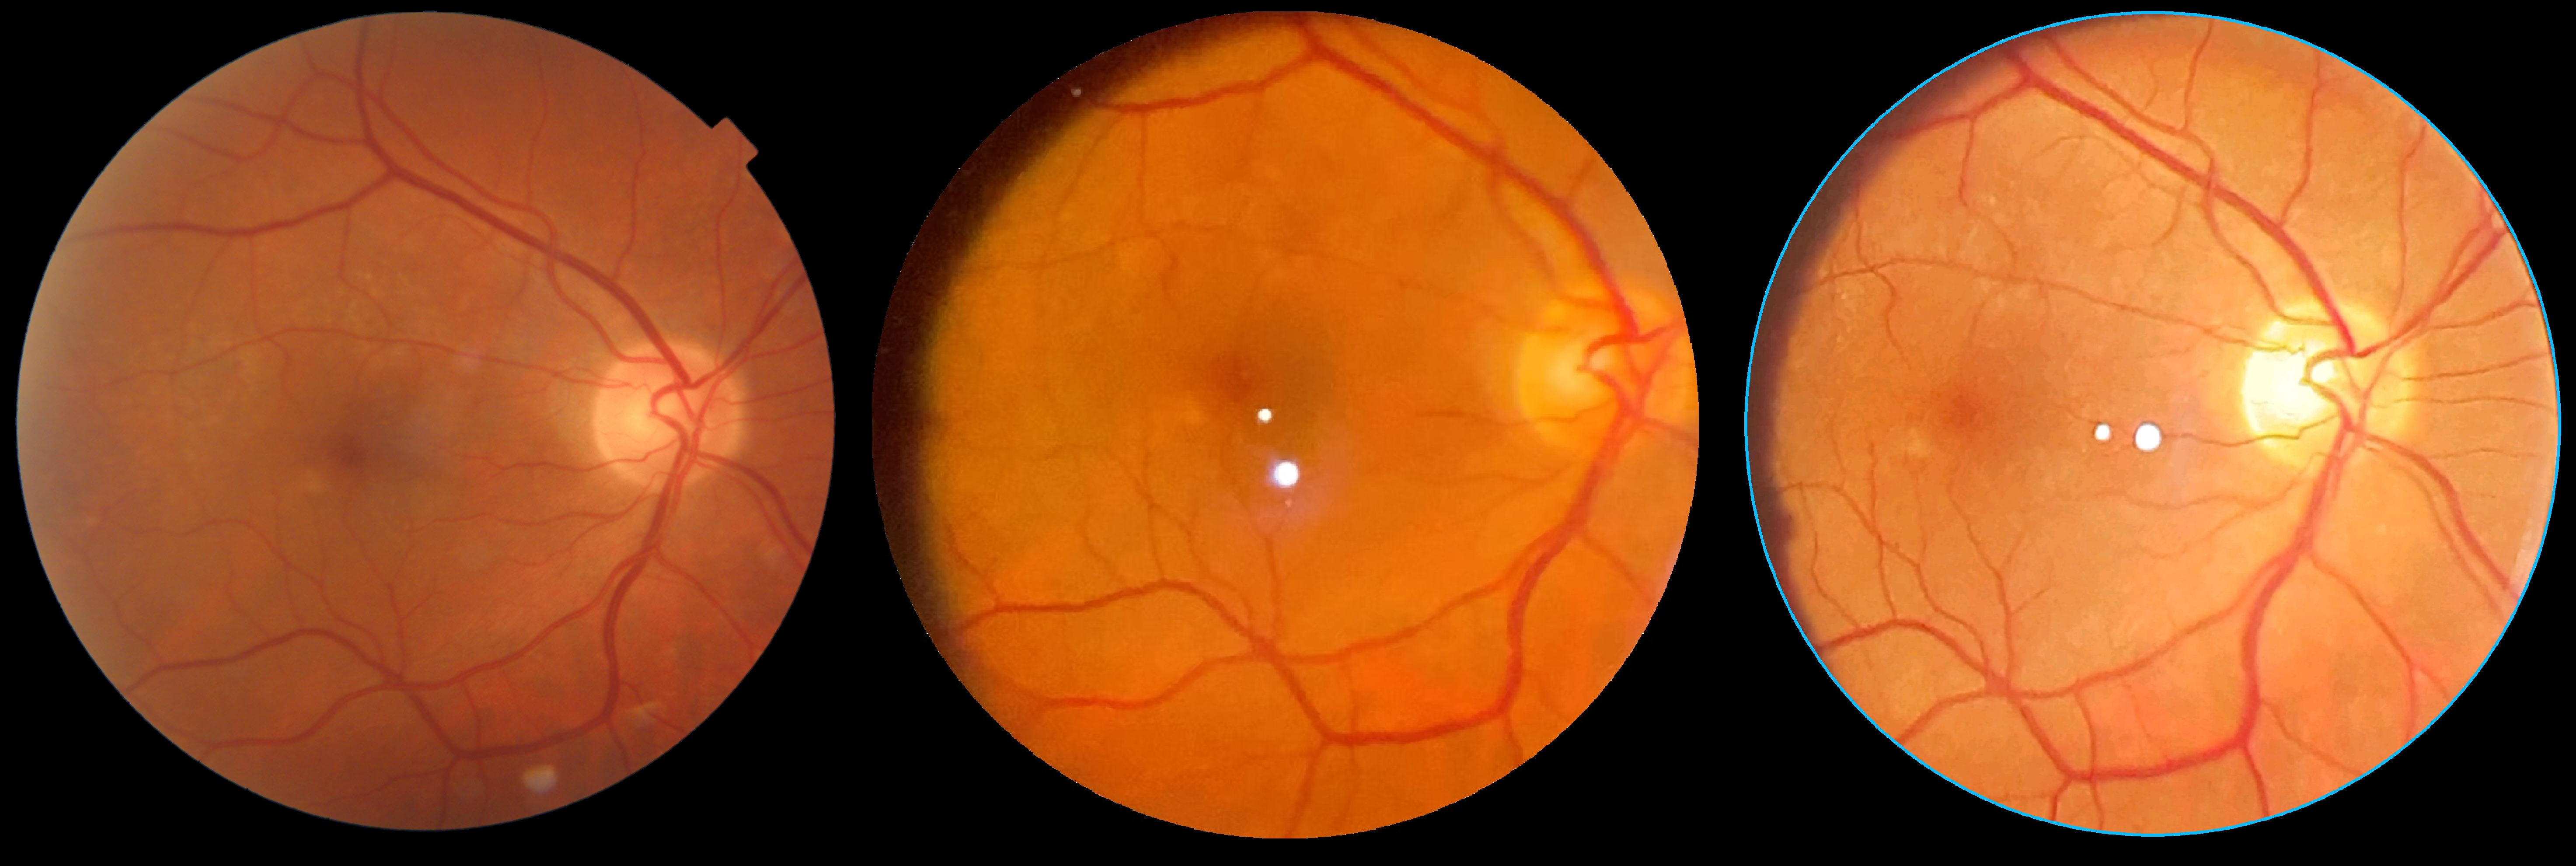
\includegraphics[width=1\textwidth]{img/dispositivos.png}
    \caption{Comparación entre 3 imágenes de retina correspondientes a un mismo ojo. La imagen de la izquierda se obtuvo usando el tomógrafo de coherencia óptica. La fotografía del centro fue tomada usando un dispositivo iPhone. La imagen de la derecha se obtuvo con un dispositivo Samsung. Fuente propia.}
    \label{fig:comp_dispositivos}
\end{figure}

\subsection{Datos de repositorios públicos}

Debido al escaso número de imágenes disponibles en la cohorte local descrita en el apartado anterior, y teniendo en cuenta que los modelos basados en \textit{Deep Learning} suelen requerir cientos o miles de muestras para desarrollar modelos que funcionen con precisión en nuevos datos, se han explorado y utilizado en este trabajo otras cohortes de imágenes de fondo de ojo públicas y conocidas para entrenar los modelos propuestos. A continuación se describen estas cohortes y sus principales características:

\begin{itemize}[itemsep=0.25em]
    \item \textbf{Kaggle}\footnote{Available at: \url{https://www.kaggle.com/competitions/diabetic-retinopathy-detection/overview}}. Se trata de una colección de 32926 fotografías de fondo de ojo en color de alta resolución utilizadas para detectar RD. Incluye imágenes de pacientes diabéticos y no diabéticos, con distintos grados de RD. El conjunto de datos está etiquetado categóricamente con etiquetas desde la ausencia de RD (grado 1) hasta PRD (grado 5). Este conjunto de datos se utiliza habitualmente para desarrollar y evaluar algoritmos de \textit{Machine Learning} (ML) para la detección automática de la RD \cite{datos:kaggle}.
    \item \textbf{DeepDRiD}\footnote{Available at: \url{https://github.com/deepdrdoc/DeepDRiD}}. Se trata de una colección de 2000 imágenes de retina seleccionadas específicamente para la tarea de detección de RD obtenidas de pacientes diabéticos mediante diferentes modalidades y dispositivos de imagen. Al igual el conjunto de datos de Kaggle y la cohote local, DeepDRiD está etiquetado categóricamente con etiquetas que abarcan desde la ausencia de RD (grado 1) hasta PRD (grado 5). Este conjunto de datos también se utiliza ampliamente en la investigación para desarrollar y evaluar algoritmos de ML para la detección automatizada y la clasificación de RD \cite{datos:deepdrid}.
    \item \textbf{Zenodo}\footnote{Available at: \url{https://zenodo.org/record/4891308##.ZEaOEHZByUn}}. Se trata de una colección de 1437 imágenes de fondo de ojo en color recogidas por el Departamento de Oftalmología del Hospital de Clínicas de Paraguay. Las imágenes fueron adquiridas a través de la cámara Visucam 500 de la marca Zeiss y etiquetadas por oftalmólogos expertos en siete categorías diferentes. Estas etiquetas fueron mapeadas a las utilizadas en nuestra cohorte local española de la siguiente manera: la categoría 1 (sin signos de RD) se asigna al grado 1; la categoría 2 (NPDR leve) se asigna al grado 2; la categoría 3 (NPDR moderado) se asigna al grado 3; las categorías 4 y 5 (NPDR severa y muy severa) se asignan al grado 4; y las categorías 6 y 7 (PDR y PDR avanzado) se asignan al grado 5. Al igual que los conjuntos de datos anteriores, éste también se utiliza en la investigación para desarrollar y evaluar algoritmos de ML destinados a predecir con precisión la RD a partir de imágenes del fondo de ojo \cite{datos:zenodo}.
\end{itemize}

Por último, la tabla \ref{tab:repositorios} resume el tamaño de cada conjunto de datos, así como la distribución de clases tanto individualmente dentro de cada conjunto de datos como globalmente considerando todos los conjuntos de datos juntos, lo que muestra claramente un problema de clasificación muy desequilibrado.

\begin{table}[]
\centering
\begin{tabular}{@{}llllll|l@{}}
\toprule
\rowcolor[HTML]{C0C0C0}
         & G1    & G2   & G3   & G4   & G5   & Total \\ \midrule
Kaggle   & 23610 & 2443 & 5292 & 873  & 708  & 32926 \\
DeepDRiD & 914   & 222  & 398  & 354  & 112  & 2000  \\
Zenodo   & 711   & 6    & 110  & 349  & 261  & 1437  \\ \midrule
Total    & 25235 & 2671 & 5800 & 1576 & 1081 & 36363 \\ \bottomrule
\end{tabular}
\caption{Distribución de las imágenes de los repositorios entre los distintos dispositivos (filas) y grados (columnas).}
\label{tab:repositorios}
\end{table}

\titlespacing{\section}{0pt}{0.25cm}{0.15cm}
\section{Herramientas}

En esta sección se describen las herramientas utilizadas en este proyecto para tratar de desarrollar una CNN capaz de detectar el grado de RD a partir de imágenes de fondo de ojo obtenidas mediante un móvil.

\subsection{Entornos de desarrollo}

\subsubsection{Anaconda}

Para el desarrollo del proyecto se ha empleado la plataforma Anaconda, debido a que está diseñado especialmente para el trabajo con Python y el análisis de datos. Anaconda está formada por dos componentes principales: Anaconda Navigator y Anaconda Prompt. En este proyecto se hizo uso mayoritariamente del primero de ellos, ya que proporciona una interfaz gráfica fácil de comprender para el usuario y numerosas herramientas para el desarrollo de código \cite{met:anaconda}. La versión de Anaconda utilizada es la 22.9.0.

De entre las distintas herramientas proporcionadas por Anaconda Navigator se optó por emplear Jupyter Notebook. Un \textit{Notebook} es un documento .json formado por una serie de celdas que pueden contener código o texto en formato \textit{markdown}. La ventaja que proporcionan es que la ejecución del código de cada celda es independiente de las demás, lo que permite probar pequeños fragmentos de código sin necesidad de ejecutar ni comprometer el resto del programa. Una vez finalizado el código, este se puede exportar como un \textit{script} de Python para su ejecución directamente desde la terminal del sistema \cite{met:paper_anaconda}.

Para mayor información sobre Anaconda y Jupyter Notebook consultar la página web: \url{https://www.anaconda.com/}.

\subsection{Lenguajes}

\subsubsection{Python}

Python es uno de los lenguajes de programación de alto nivel más versátil, potente y empleado a nivel mundial en la actualidad \cite{met:demanded}. Es un lenguaje interpretado, no compilado, lo que agiliza enormemente el desarrollo del código y de la experimentación \cite{met:deepl_py}. La versión utilizada es la 3.9.12.

Se ha escogido Python para el proyecto por ser especialmente apropiado para el desarrollo de código en el contexto de \textit{Deep Learning}, además de proporcionar una gran variedad de bibliotecas y paquetes para este desarrollo. Otra de las ventajas que proporciona Python es la documentación y la comunidad que lo respalda, lo que facilita la identificación y resolución de problemas \cite{met:deepl_py}. 

Además Python ha sido el lenguaje de programación más utilizado a lo largo de nuestro recorrido en el grado. Es por ello que el dominio y conocimiento que tengo acerca de esta herramienta es mayor que el manejo de cualquier otro lenguaje de programación.

Para mayor información acerca de Python: \url{https://www.python.org/}

\subsubsection{\LaTeX}

Se ha empleado LaTeX para la elaboración de la memoria. Este lenguaje era el establecido por la coordinación del Trabajo de Fin de Grado para la elaboración de la memoria. LaTeX permite realizar documentos de alta calidad tipográfica, gracias a la versatilidad que ofrece en el código. Además facilita la gestión de referencias bibliográficas, así como la portabilidad de los documentos. 

Para la redacción de la memoria se empleó el editor colaborativo Overleaf. Para mayor información sobre el lenguaje LaTeX consultar: \url{https://www.latex-project.org/}. Para mayor información sobre el editor Overleaf consultar: \url{https://es.overleaf.com/learn}.

\subsubsection{Shell scripting}

Este lenguaje es empleado para escribir secuencias de comandos que se desean ejecutar en el intérprete de comandos del sistema operativo de un equipo. En mi caso se empleó para poder ejecutar aquellos los archivos necesarios en el Supercomputador de Castilla y León (SCAYLE). El shell empleado en mi caso fue Bash (Bourne Again SHell), que es el más comúnmente utilizado en sistemas Unix y Linux (como es el caso de SCAYLE) \cite{met:bash}. 

El uso de este tipo de código fue necesario en  SCAYLE para el manejo de archivos, la activación/desactivación de entornos, ejecución de archivos de Python o configuración de parámetros de ejecución (GPU o CPU, número de nodos reservados, cantidad de memoria RAM reservada, tiempo máximo de ejecución...).

\subsubsection{Markdown}

Markdown es una herramienta gratuita de marcado ligero que permite crear contenido de una manera sencilla de escribir. Se emplea para dar formato a textos e imágenes mediante una sintáxis programática bastante sencilla. El código Markdown se escribe como texto plano, pero al realizar su ejecución se visualiza con el formato deseado. 

En este proyecto se usó Markdown para modelar la página principal del repositorio de GitHub en el que se almacena toda la información del trabajo.

Puede encontrarse más información acerca de Markdown en la web: \url{https://markdown.es/}.

\subsection{Bibliotecas}

A continuación se van a mencionar y explicar las principales bibliotecas empleadas en el desarrollo del proyecto. Una biblioteca (o \textit{library}) en programación es un conjunto de código predefinido que proporciona funciones, clases y estructuras de datos para llevar a cabo tareas relacionadas con un determinado propósito \cite{met:libreria}. Todas las bibliotecas que se han empleado en este código pueden encontrarse en el repositorio del entorno Anaconda o en el repositorio PyPI (\textit{Python Package Index}), por lo que pueden ser fácilmente instaladas en el equipo.

\subsubsection{\texttt{torch}}

Este paquete contiene las estructuras de datos para definir y almacenar los tensores además de funciones para operar matemáticamente sobre esos tensores. 

Dentro de esta biblioteca se empleó exhaustivamente el paquete \texttt{torch.nn}, que proporciona los distintos métodos y capas para la creación de CNN, así como las funciones de optimización y de pérdida necesarias para el entrenamiento de los modelos. Además en el paquete \texttt{torch.nn} se encuentra la clase \texttt{Module} que constituye la superclase de la que heredan todas las arquitecturas creadas. Toda la documentación puede encontrarse en el siguiente enlace: \url{https://pytorch.org/docs/stable/nn.html}.

También se debe mencionar el paquete \texttt{torch.utils.data} que permite acceder a la estructura \texttt{DataLoader}, fundamental para poder cargar las imágenes de los distintos directorios en memoria y así poder entrenar los modelos. Su respectiva documentación puede encontrarse en: \url{https://pytorch.org/docs/stable/data.html}.

\subsubsection{\texttt{Torchvision}}

Se trata de una biblioteca que incorpora conjuntos de datos conocidos (como MNIST, ImageNet o CIFAR10), arquitecturas ya predefinidas o funciones para la importación y transformación de imágenes. En el proyecto se empleó principalmente para redimensionar y normalizar las imágenes mediante el módulo \texttt{torchvision.transforms}, y para definir la ruta en la que se encontraban las imágenes empleando \texttt{torchvision.datasets.ImageFolder}. La documentación puede encontrarse en: \url{https://pytorch.org/vision/stable/index.html#module-torchvision}.

\subsubsection{\texttt{Matplotlib}}

\texttt{Matplotlib} es una biblioteca para la creación de visualizaciones estáticas, animadas e interactivas en Python. Incorpora numerosas funciones para la representación de gráficas e imágenes, permitiendo controlar distintos parámetros y opciones a la hora de representar estas figuras. En el proyecto se empleó para representar las gráficas de \textit{accuracy} y \textit{loss} de los distintos modelos. La documentación está disponible en: \url{https://matplotlib.org/}.

\subsubsection{\texttt{NumPy}}

Es una de las bibliotecas más empleadas y conocidas de Python. Proporciona soporte para crear vectores y matrices, así como funciones para poder operar con estas estructuras y otras funciones matemáticas de muy alto nivel. En el proyecto se emplea para la creación de matrices para almacenar las métricas y predicciones en la evaluación de los modelos. La documentación puede encontrarse en: \url{https://numpy.org/}.

\subsubsection{\texttt{time}}

Se trata de un módulo que incorpora funciones que permiten consultar información relacionada con el tiempo (fecha, tiempo transcurrido, conversiones entre formatos de fecha) así como algunas funciones que permiten detener la ejecución de un programa durante un número determinado de segundos. En el trabajo desarrollado únicamente se empleó una función, \texttt{time.time()}, que devuelve los segundos que han transcurrido desde el 1 de enero de 1970. De manera que se invocó antes y después del entrenamiento de un modelo para, restando el resultado de ambas invocaciones, conocer el tiempo dedicado al entrenamiento. Más información en: \url{https://docs.python.org/3/library/time.html#time.time}.

\subsubsection{\texttt{Pillow}}

Este paquete proporciona las funciones y estructuras necesarias para el procesamiento y manejo de imágenes en Python. Está diseñado para permitir un acceso rápido a los datos y un almacenamiento de las imágenes empleando el menor espacio posible. En nuestro caso únicamente se va a emplear el paquete \texttt{PIL.ImageFile}, para permitir el uso de imágenes truncadas (como es el caso de algunas imágenes almacenadas en los directorios) y algunas funciones de este módulo para el preprocesamiento de las imágenes. Más información en: \url{https://pillow.readthedocs.io/en/stable/reference/ImageFile.html}.

\subsubsection{\texttt{pandas}}

Se trata de otra de las bibliotecas más habituales en Python. Está enfocada en la manipulación y análisis de datos, ofreciendo estructuras de datos como \texttt{DataFrame} que permiten albergar datos estructurados o seemi-estructurados como ficheros .csv, Excel o bases de datos SQL. El uso de este paquete en el proyecto se ha limitado a la manipulación del archivo Excel proporcionado como parte del conjunto de datos de la cohorte local. Puede obtenerse más información en la siguiente dirección: \url{https://pandas.pydata.org/docs/user_guide/index.html#user-guide}.

\subsubsection{\texttt{os}}

Este módulo proporciona funciones relacionadas con el sistema operativo del equipo, tales como la manipulación de archivos, obtención de rutas o creación/eliminación de directorios. Se ha empleado para la organización de las imágenes en el proceso de depuración de datos así como para la creación de directorios. Más información en: \url{https://docs.python.org/3/library/os.html}.

\subsubsection{\texttt{seaborn}}

\texttt{Seaborn} es una biblioteca para la visualización de datos y gráficas basada en la anteriormente mencionada \texttt{Matplotlib} y fácilmente integrable con \texttt{pandas}. Permite realizar visualizaciones de gráficas y resultados de más alto nivel. Fue empleada para la creación de las matrices de confusión de algunos modelos. Más información en: \url{https://seaborn.pydata.org/}.

\subsubsection{\texttt{Scikit-learn}}

Esta biblioteca está diseñada para facilitar las tareas de aprendizaje automático. Incluye por tanto distintos modelos de \textit{Machine Learning}, así como funciones para llevar a cabo el entrenamiento y evaluación de dichos modelos. En este proyecto se ha empleado el módulo \texttt{sklearn.metrics} que incorpora las distintas funciones necesarias para la obtención de las métricas (\texttt{accuracy\_score, f1\_score, confusion\_matrix}...), tanto del \textit{baseline} como del rendimiento de los distintos modelos. Puede encontrarse más información en la siguiente dirección: \url{https://scikit-learn.org/stable/modules/model_evaluation.html}.

\subsubsection{\texttt{OpenCV}}

Se trata de un paquete desarrollado específicamente para las tareas de visión artificial. Entre sus funciones se incluyen distintos métodos que permiten modificar las imágenes, aplicar filtros o utilizar herramientas de inteligencia artificial para el reconocimiento automático de formas o figuras en las imágenes. En el proyecto es empleado en las tareas de preprocesamiento e \textit{inpaint} de las imágenes. Para más información: \url{https://opencv.org/}.

\subsubsection{\texttt{Scikit-Image}}

\texttt{Scikit-Image} es una colección de algoritmos diseñados para el procesamiento de imágenes. Incorpora funciones para la modificación de imágenes, su manipulación dentro del equipo y su impresión en pantalla, así como métodos para el reconocimiento de formas o la aplicación de filtros. En el proyecto se empleó para la detección de los destellos de flash en las imágenes y así poder aplicar el \textit{inpainting}. Para más información: \url{https://scikit-image.org/}.

\subsubsection{\texttt{shutil}}

Este paquete incorpora funciones que permiten operar a alto nivel con archivos y colecciones de archivos. Especialmente ofrece operaciones que dan soporte a la copia de archivos. En el proyecto se empleó para la organización de las imágenes en los distintos directorios. Para más información: \url{https://docs.python.org/es/3/library/shutil.html}.

\subsection{Marco de trabajo}

El marco de trabajo hace referencia al conjunto de herramientas, criterios y conceptos que se emplean para enfrentar una determinada tarea. En este caso, cuando hablamos de marco de trabajo me refiero al entorno de programación que se va a emplear y las bibliotecas que se van a usar. En mi caso se trabajará con PyTorch.

PyTorch es una herramienta ampliamente utilizada en el desarrollo de proyectos de redes neuronales. Se trata de una biblioteca científica (un conjunto de funciones prediseñadas y de estructuras de datos) de código abierto desarrollada por Facebook en 2016 y basada en el lenguaje de programación Python \cite{marco:pytorch_libro}. Esta biblioteca nos va a permitir construir los modelos de CNN de una manera más sencilla, así como crear las estructuras y herramientas necesarias para poder llevar a cabo el entrenamiento y validación de estos modelos \cite{marco:pytorch}.

Se ha seleccionado este marco de trabajo debido a las ventajas que presenta en comparación con otros posibles entornos como TensorFlow. PyTorch es sencillo de entender, permite utilizar el depurador de código de Python y está diseñado para ser ejecutado en unidades de procesamiento gráfico (GPU), por lo que el código se ejecutará más rápidamente \cite{marco:pytorch_libro}. Además es una herramienta de desarrollo de redes neuronales más enfocada a la investigación y especialmente en el campo de la visión por computador \cite{marco:pytorch}.

La abstracción básica de PyTorch, la estructura de datos sobre la que se sustenta esta biblioteca y que se emplea para almacenar todo tipo de datos, se denomina \textit{tensor} \cite{marco:pytorch_libro}. Un tensor no es más que una matriz multidimensional que almacena en su interior elementos del mismo tipo (generalmente números decimales) \cite{marco:pytorch_web}. Siendo muy reduccionistas, podríamos afirmar que toda la computación realizada por PyTorch se puede definir como creación de tensores y operaciones con ellos \cite{marco:pytorch_libro}.

\subsection{Metodología}

\subsubsection{CRISP-DM}

\textit{CRISP-DM}, siglas que aluden a los términos \textit{CRoss Industry Standard Process for Data Mining}, es una estrategia aplicable a múltiples ámbitos de la industria, pero especialmente empleada en la minería de datos \cite{crispdm:azevedo}, que consiste en 6 fases o etapas iterativas que abarcan desde la comprensión del ámbito en que se va a trabajar (o comprensión del negocio si se traduce directamente del inglés \textit{Business Understanding}), hasta el despliegue de los resultados \cite{crispdm:niaksu,crispdm:schorer}.

Las 6 fases que constituyen el modelo son las siguientes \cite{crispdm:niaksu,crispdm:schorer}:
\begin{enumerate}[itemsep=0.1em]
    \item Comprensión del ámbito o negocio (\textit{Business understanding}).
    \item Comprensión de los datos (\textit{Data understanding}).
    \item Preparación de los datos (\textit{Data preparation}).
    \item Modelado (\textit{Modeling}).
    \item Evaluación (\textit{Evaluation}).
    \item Despliegue o implementación (\textit{Deployment}).
\end{enumerate}

Como se ha mencionado anteriormente, \textit{CRISP-DM} es una metodología iterativa, es decir, estas 6 etapas se van repitiendo en un bucle cuyo orden no está rígidamente definido, sino que la sucesión de las distintas fases estará determinada por el resultado de la etapa finalizada \cite{crispdm:niaksu}.

En el anexo \textit{Plan de Proyecto Software} se explica más en detalle esta metodología, así como sus fases.

\subsubsection{ZenHub}

ZenHub es una herramienta de gestión de proyectos que permite organizar las tareas y realizar un seguimiento del desarrollo del trabajo. Una de sus grandes ventajas es su fácil integración con GitHub, permitiendo la creación de etiquetas para agrupar las tareas, crear \textit{sprints}, asignar cada labor a un usuario concreto o estimar el esfuerzo requerido por cada tarea. Entre sus características más relevantes, han sido de especial ayuda e interés el Tablero Kanban que permite organizar de manera sencilla las tareas pendientes, la estimación de esfuerzo de cada tarea y los \textit{Reports}, que permiten observar la evolución del trabajo de manera más visual.

En este trabajo se empleó ZenHub para implementar la metodología CRISP-DM descrita en el apartado anterior. Para más información acerca de esta implementación puede consultarse el anexo \textit{Plan de Proyecto Software}.

Para más información acerca de ZenHub puede visitarse la página web: \url{https://www.zenhub.com/}.

\subsection{Repositorio}

Para la elaboración del repositorio online en el que se encuentra toda la información del proyecto, incluida la memoria, las imágenes y los archivos de código, se empleó la plataforma GitHub. Para la sincronización entre el equipo local y el repositorio online se utilizó la herramienta GitHub Desktop.

\subsubsection{GitHub}

GitHub es la plataforma en línea que permite alojar, administrar y colaborar en proyectos de desarrollo de software. Es la plataforma más empleada para este tipo de propósitos, con más de 100 millones de desarrolladores, 4 millones de organizaciones y 300 millones de repositorios. Permite a distintos usuarios participar conjuntamente en la elaboración de un mismo proyecto de código, incorporando un sistema de control de versiones para realizar un seguimiento a los cambios realizados.

Para más información sobre esta herramienta, visitar el enlace: \url{https://github.com/about}. 

\subsubsection{GitHub Desktop}

GitHub Desktop es una herramienta de código abierto, desarrollada por la propia organización de GitHub, que permite sincronizar el equipo local y el repositorio online que se desee. Mediante el uso de esta herramienta, podemos trabajar con los archivos en nuestro ordenador, realizando las modificaciones necesarias, y posteriormente actualizar el contenido del repositorio online para incluir las nuevas modificaciones.

Para más información visitar el enlace: \url{https://docs.github.com/en/get-started/using-github/github-desktop}. 

\subsection{Otras herramientas}

\subsubsection{Zotero}

Zotero es un gestor de referencias bibliográficas gratuito. La aplicación cuenta con una base de datos interna en la que almacena la bibliografía que se desee, usando el convenio que se indique. Incluye una extensión para Google Chrome (Zotero Connector) que permite añadir a la base de datos de referencias la página web que se esté visitando. 

Se trata de una herramienta muy intuitiva y sencilla de manejar que permite gestionar las referencias de forma clara y ordenada. En el caso de este proyecto, Zotero fue empleado para obtener el BibTeX (formato de referencia bibliográfica requerido por LaTeX) de las páginas web visitadas. 

Para más información se puede consultar la dirección: \url{https://www.zotero.org/}.

\subsubsection{PuTTY}

PuTTY es un programa de código abierto que proporciona una implementación de cliente SSH (Secure SHell) para Windows y Unix. Se trata de una aplicación que permite establecer conexiones remotas y seguras entre equipos mediante el protocolo SSH.

El programa proporciona una interfaz similar al símbolo del sistema de Windows, de manera que permite realizar funciones básicas del sistema operativo del equipo remoto desde el equipo local (listado de archivos, ejecución de instrucciones, cambio de directorios...).

En el proyecto se empleó esta aplicación para poder conectarme al servidor de SCAYLE. Para ello desde la página de SCAYLE se proporciona una URL y un número de puerto, que deben introducirse al iniciar PuTTY. Tras introducir el usuario y contraseña de SCAYLE, ya se tiene acceso a la partición reservada para mí, lo que me permite modificar o leer archivos, moverlos entre directorios o ejecutarlos \cite{met:putty}.

Para obtener más información sobre PuTTY visite la dirección: \url{https://the.earth.li/~sgtatham/putty/0.78/htmldoc/}.

\subsubsection{WinSCP}

WinSCP es una herramienta de software libre para Windows que emplea el protocolo SCP (\textit{Secure Copy}) para la transferencia de datos entre un equipo local y un servidor remoto. Ofrece una interfaz muy sencilla, dividida en dos pantallas (una representa nuestro equipo local con sus directorios y otra el equipo remoto), que permite enviar y descargar archivos en un equipo remoto simplemente arrastrando los archivos de una pantalla a otra. 

En el proyecto se empleó para cargar los \textit{scripts} e imágenes deseados en el servidor de SCAYLE, así como para descargar los archivos de resultados correspondientes. Para conectar el equipo local y remoto, desde SCAYLE se proporciona una URL y un número de puerto, de esta manera únicamente debemos introducir nuestro usuario y contraseña en la aplicación y ya podremos realizar la transferencia de archivos \cite{met:winscp}. Aunque es una herramienta muy útil, para realizar transferencias de grandes cantidades de datos no es la más adecuada. En esos casos es más apropiado emplear el comando \texttt{rsync}\footnote{Esta instrucción se explica más detalladamente en el anexo \textit{Estudio experimental}}.

Para más información sobre WinSCP visite el enlace: \url{https://winscp.net/eng/docs/introduction}.

\section{Técnicas}

En esta sección se van a describir las técnicas empleadas en el desarrollo del proyecto. Se explicará el objetivo perseguido con la técnica y el procedimiento de realización de la misma.

\subsection{\textit{Early Stopping}}

Cuando se entrena una red neuronal uno de los aspectos que se debe evitar es el sobreentrenamiento de dicha red, es decir, se debe tratar de impedir que el modelo se especialice tanto en los datos de entrenamiento que pierda la capacidad de generalización, y por tanto su capacidad de dar resultados correctos a partir de datos nunca antes vistos \cite{early:butwhen}. Existen distintas estrategias para tratar de solventar este problema, por ejemplo el uso de conjuntos de datos más grandes, la simplificación del modelo o la inclusión de las ya mencionadas capas de regularización como \textit{Dropout} \cite{early:overview}. Sin embargo, para la realización del proyecto se ha optado por la estrategia denominada \textit{early stopping}.

El \textit{early stopping} consiste en finalizar el entrenamiento de la red una vez se considere que el modelo ha dejado de aprender y comienza a sobreentrenar, evitando así que el modelo siga entrenando y pierda esa capacidad de generalización. Conforme pasan las épocas, la red mejora su rendimiento utilizando datos entrenados, por lo que el error de la red sobre estos datos no puede emplearse para determinar el \textit{early stopping}. Para establecer el punto de inflexión se emplea el error de la red al clasificar un conjunto denominado de \textit{validación} \cite{early:butwhen}.

Este conjunto de validación se corresponde con un porcentaje de los datos de entrenamiento originales que se reservan y no se emplean en el entrenamiento, es decir, son datos nuevos para el modelo (pero sin ser datos de evaluación). De esta manera, tras cada época de entrenamiento, se le proporcionará a la red el conjunto de datos de validación para obtener las etiquetas correspondientes y así poder monitorizar el error sobre este conjunto \cite{early:overview}. 

El momento en el que el error empleando los datos de validación comience a incrementar representará idealmente el punto donde el modelo comienza a sobreentrenar. Digo idealmente ya que el error en las predicciones usando datos de validación no suele presentar un único mínimo relativo, sino que que en ocasiones es similar a lo observado en la figura \ref{fig:validacion}, una gráfica con distintos cambios de sentido \cite{early:butwhen}. Por ello se suele establecer un número de épocas de ``paciencia'', es decir, el número de épocas en las cuales si el modelo no logra disminuir el mínimo valor de error de validación conseguido hasta el momento, se activa la herramienta \textit{early stopping} finalizando el entrenamiento.

\begin{figure}[h]
    \centering
    \includegraphics[width=0.75\textwidth]{img/validacion error.png}
    \caption{Gráfica de la evolución del error de validación. Eje vertical: valor del error de validación. Eje horizontal: número de épocas de entrenamiento \cite{early:butwhen}.}
    \label{fig:validacion}
\end{figure}

En el caso de este proyecto en cuestión, la división de los datos entre entrenamiento y validación fue del 80\% y 20\% de los disponibles (sin considerar aquellos reservados para evaluación) respectivamente. El número de épocas de paciencia establecido fue 7. Esto significa que si transcurridas 7 épocas no se ha logrado descender el valor del error de validación por debajo del mínimo obtenido hasta el momento, el entrenamiento finaliza, recuperándose el estado del modelo en el punto en que se alcanzó dicho mínimo. Si se logra descender dicho valor, se iniciarán nuevamente las épocas de paciencia y así sucesivamente.

\subsection{Preprocesamiento}

Con el objetivo de mejorar el rendimiento de las CNN creadas, y siguiendo la línea de trabajo de otros autores \cite{preproc:detection, preproc:maison}, se desarrolló un \textit{pipeline} para preprocesar las imágenes de fondo de ojo empleadas en el entrenamiento y evaluación de los modelos.

El propósito del preprocesamiento es homogeneizar el aspecto de todas las imágenes (especialmente aquellas procedentes de distintos repositorios) y destacar las características más diferenciadoras de la retina, eliminando los detalles menos relevantes y facilitando el aprendizaje de los modelos. 

El preprocesamiento consta de 2 etapas:

\begin{itemize}[itemsep=0.25em]
    \item Recorte circular. En la mayor parte de las imágenes obtenidas de los repositorios descritos en la sección \textit{Descripción de los datos} las fotografías de fondo de ojo se encuentran enmarcadas en un fondo negro, que no proporciona ninguna información relevante para el modelo. Es por ello que el primer paso es realizar un recorte circular de las imágenes, ajustando los bordes de las mismas hasta la circunferencia que compone el fondo de ojo, tal y como se describe en \cite{preproc:kaggle}, eliminando así las regiones negras no informativas.

    Para la realización de este paso se genera una máscara de cada imagen, considerando como condición para la máscara que el píxel evaluado tenga un valor superior a un valor establecido como parámetro (próximo a 0, para así evitar aquellos píxeles negros o muy oscuros). Por lo tanto, es necesaria una conversión previa de la imagen a escala de grises \cite{preproc:kaggle}.
    
    \item Filtro gaussiano. Una vez se ha ajustado el borde de la imagen, se aplica sobre la imagen un filtro Gaussiano mediante la combinación de las funciones \texttt{cv2.addWeighted()} y \texttt{cv2.GaussianBlur()}, ambas dos de la biblioteca \texttt{OpenCV}, según se describe en \cite{preproc:kaggle}. El objetivo de este preprocesamiento es resaltar la morfología de los vasos sanguíneos que irrigan la retina, así como las posibles características relevantes como hemorragias o exudados \cite{preproc:maison}. 

    El filtro gaussiano suaviza las imágenes, eliminando así el ruido y los pequeños detalles, permitiendo que destaquen el resto de elementos. Su funcionamiento se basa en una matriz de dimensiones $n*n$ cuyos valores siguen una distribución gaussiana. Esta matriz convoluciona sobre la imagen que se desea preprocesar, logrando así el efecto deseado \cite{preproc:ieee}.
\end{itemize}

En la figura \ref{fig:preproc} se puede observar el resultado de este preprocesamiento sobre una imagen de fondo de ojo tomada con un dispositivo Samsung, otra tomada con un tomógrafo de coherencia óptica y una imagen de fondo de ojo correspondiente al repositorio Zenodo.

\begin{figure}[!t]
\centering

\begin{subfigure}[t]{0.3\textwidth}
  \includegraphics[width=\textwidth]{img/samsung.png}
\end{subfigure}
\begin{subfigure}[t]{0.3\textwidth}
  \includegraphics[width=\textwidth]{img/OCT.jpg}
\end{subfigure}
\begin{subfigure}[t]{0.3\textwidth}
  \includegraphics[width=\textwidth]{img/zenodo.jpg}
\end{subfigure}

\vspace{0.3cm} % Espacio vertical entre filas

\begin{subfigure}[t]{0.3\textwidth}
  \includegraphics[width=\textwidth]{img/samsung_proc.png}
\end{subfigure}
\begin{subfigure}[t]{0.3\textwidth}
  \includegraphics[width=\textwidth]{img/OCT_proc.jpg}
\end{subfigure}
\begin{subfigure}[t]{0.3\textwidth}
  \includegraphics[width=\textwidth]{img/zenodo_proc.jpg}
\end{subfigure}

\caption{Comparación entre imágenes originales y preprocesadas. Todas las imágenes se corresponden con un ojo izquierdo diagnosticado con grado 3 (NPDR moderada). La imagen superior izquierda se corresponde con la original tomada con Samsung, la imagen inferior izquierda es la imagen obtenida con Samsung preprocesada. La imagen superior central ha sido obtenida con el OCT, la imagen inferior central se corresponde con la imagen de OCT preprocesada. La imagen superior derecha es la imagen original obtenida del repositorio Zenodo, la imagen inferior derecha es la imagen del repositorio Zenodo preprocesada. Fuente propia.}
\label{fig:preproc}
\end{figure}

\subsection{\textit{Inpainting}}

Como se puede observar en las imágenes adquiridas con teléfonos móviles (ya sea Samsung o iPhone), existen dos puntos blancos en el centro de la imagen que se corresponden con el destello del flash de la cámara del teléfono. Este destello es más evidente y marcado cuando la imagen es preprocesada siguiendo la técnica descrita en el apartado anterior. Un claro ejemplo puede observarse en la figura \ref{fig:preproc}, en las imágenes de la columna izquierda.

He considerado que dicho destello puede ocasionar efectos no deseados en los modelos, especialmente si este flash se encuentra únicamente en las imágenes obtenidas con Samsung o iPhone. Es por ello que se plantea la opción de realizar el \textit{inpainting} de estas imágenes, para eliminar artificialmente ese destello.

El inpainting es una técnica que originalmente busca restaurar la parte dañada de los píxeles de una imagen incompleta para posteriormente reconstruir y generar una aproximación de la imagen original \cite{inp:review}. En este caso, la técnica se aplicaría con el objetivo de eliminar el destello y generando una nueva imagen que sea lo más parecida a la original.

Existen distintas aproximaciones para sustituir el valor de aquellos píxeles que se desean eliminar, pero he optado por el inpaint biarmónico, basado en el principio del biarmónico. Este método aborda el proceso como una ecuación de Laplace modificada, que se va resolviendo mediante iteraciones. El objetivo perseguido es que la sustitución de los valores de los píxeles sea suave y coherente \cite{inp:biharmo}. En este proceso de inpainting, una vez sustituidos los valores de los píxeles, tienen lugar una serie de iteraciones con el objetivo de suavizar los bordes y ajustar los detalles.

La técnica de inpainting aplicada en el proyecto consiste en un proceso de varios pasos, y fue diseñada empleando como guion los ejemplos proporcionados en la documentación de las funciones usadas:

\begin{itemize}
    \item En primer lugar, se generó la máscara correspondiente a los puntos de luz del flash. Para ello, se aplicó la función \texttt{HoughCircles} del paquete \texttt{OpenCV}\footnote{Disponible en: \url{https://docs.opencv.org/4.x/da/d53/tutorial_py_houghcircles.html}} a la imagen previamente convertida a blanco y negro y desenfocada.
    
    \item De todos los círculos detectados por esta función, sólo se seleccionaron para la máscara aquellos cuyo radio no fuera superior a 1/53 de la anchura de la imagen y que estuvieran situados en el centro de la misma, considerando como centro todos los píxeles ubicados entre los 11/30 y 18/30 de la vertical, y los 13/30 y 17/30 de la horizontal de la imagen.

    \item Una vez obtenida la máscara, se realizó un inpainting biarmónico mediante la función incluida en el módulo \texttt{restoration.inpaint} del paquete \texttt{Scikit-image}\footnote{Disponible en: \url{https://scikit-image.org/docs/stable/auto_examples/filters/plot_inpaint.html##sphx-glr-auto-examples-filters-plot-inpaint-py}} empleando dicha máscara.
\end{itemize}

En la figura \ref{fig:inp} puede observarse una comparación entre una misma imagen en sus distintas versiones: original, preprocesada, tras el inpainting y tras el inpainting y preprocesada.

\begin{figure}[!t]
\centering
\begin{subfigure}[t]{0.45\textwidth}
  \includegraphics[width=\textwidth]{img/iphone.PNG}
\end{subfigure}
\begin{subfigure}[t]{0.45\textwidth}
  \includegraphics[width=\textwidth]{img/iphone_proc.PNG}
\end{subfigure}

\vspace{0.3cm} % Espacio vertical entre filas

\begin{subfigure}[t]{0.45\textwidth}
  \includegraphics[width=\textwidth]{img/iphone_inp.PNG}
\end{subfigure}
\begin{subfigure}[t]{0.45\textwidth}
  \includegraphics[width=\textwidth]{img/iphone_proc_inp.PNG}
\end{subfigure}

\caption{Comparación entre una imagen original tomada con un iPhone 11 Pro a un ojo izquierdo diagnosticado con grado 4 (NPDR severa) y sus distintas versiones: preprocesada, tras el inpainting y tras el inpainting y preprocesada. La imagen superior izquierda se corresponde con la imagen original, la imagen inferior izquierda es la imagen original preprocesada, la superior derecha es la imagen tras el inpaint y la imagen inferior derecha es la imagen tras el inpaint y preprocesada. Fuente propia.}
\label{fig:inp}
\end{figure}
\capitulo{4}{Conclusiones} \label{Conc}

Todo proyecto debe incluir las conclusiones que se derivan de su desarrollo. Éstas pueden ser de diferente índole, dependiendo de la tipología del proyecto, pero normalmente van a estar presentes un conjunto de conclusiones relacionadas con los resultados del proyecto y un conjunto de conclusiones técnicas. 

\section{Aspectos relevantes.}

Como ya ha sido comentado en el capítulo \ref{Obj}, la principal motivación del proyecto era el desarrollo de una CNN capaz de predecir el grado de RD a partir de una imagen de fondo de ojo. Para lograr este objetivo se ha seguido una estrategia que podríamos considerar de \textit{fuerza bruta}, creando numerosas arquitecturas y probando todas las combinaciones posibles entre dichas arquitecturas y distintos conjuntos de datos de entrenamiento, para tratar de encontrar un modelo con un desempeño superior al de un oftalmólogo. 

Este apartado pretende recoger los aspectos más interesantes del \textbf{desarrollo del proyecto}, comentados por los autores del mismo.

Debe incluir los detalles más relevantes en cada fase del desarrollo, justificando los caminos tomados, especialmente aquellos que no sean triviales. 

Puede ser el lugar más adecuado para documentar los aspectos más interesantes del proyecto y también los resultados negativos obtenidos por soluciones previas a la solución entregada.

Este apartado, debe convertirse en el resumen de la experiencia práctica del proyecto, y por sí mismo justifica que la memoria se convierta en un documento útil, fuente de referencia para los autores, los tutores y futuros alumnos.

\section{Resumen de resultados.}

Breve resumen de los resultados. En caso de ser un trabajo muy experimental, los resultados completos pueden aparecer en su anexo correspondiente.

\section{Discusión.}

Discusión y análisis de los resultados obtenidos.





\capitulo{5}{Aspectos relevantes del desarrollo del proyecto} \label{Aspe}

\capitulo{6}{Lineas de trabajo futuras} \label{Fut}


Este capítulo debería ser informe crítico indicando cómo se puede mejorar el proyecto, o cómo se puede continuar trabajando en la línea del proyecto realizado.


\bibliographystyle{plain}
\bibliography{bibliografia}

\end{document}
